\documentclass{template/template}

\usepackage[T1]{fontenc} % evropské uvozovky
\usepackage{subcaption}
\usepackage{amsmath}
\usepackage{enumitem}
\usepackage{hyperref}
\usepackage{gensymb} % balíček symbolů
\usepackage{booktabs}
\usepackage{lmodern}
\usepackage{csquotes} % text lze uvést do uvozovek pomocí \enquote{text}
\usepackage{textcomp}

\usepackage[toc,page]{appendix}
\usepackage{color} % balíček pro obarvování textů
\usepackage{xcolor}  % zapne možnost používání barev, mj. pro \definecolor
\definecolor{mygreen}{RGB}{0,153,153} % nastavení barev odkazů 
\usepackage{listings} % balíček pro formátování zdrojových kódů 
\usepackage[author=,status=draft]{fixme} % vkládání poznámek  
% dva módy (status): draft (poznámky se zobrazují v PDF) / final (poznámky se nezobrazují v PDF)
\usepackage{multirow}
\usepackage{float}

\usepackage{expl3} % bibtex dependency, must be loaded prior to the bibtex
\usepackage[backend=bibtex,bibstyle=numeric,sorting=none,date=long,dateabbrev=false,texencoding=utf8,bibencoding=utf8,style=iso-numeric]{biblatex}

\usepackage[a4paper]{geometry}

\lstset { 
    language=C++,
    backgroundcolor=\color{black!5}, % set backgroundcolor
    basicstyle=\footnotesize,% basic font setting
}

\addbibresource{text.bib}
%\nocite{*}

\titlecz{Využití videonávodů pro výuku konstrukce v SolidWorks} % Název práce
\titleen{Videoguides usage in SolidWorks construction education} % Anglický název práce
\author{Petr Štourač} % Jméno autora
\institution{STŘEDNÍ PRŮMYSLOVÁ A VYŠŠÍ ODBORNÁ ŠKOLA BRNO, Sokolská 1} % Celý název instituce
\institutiontype{příspěvková organizace} % Typ instituce
\thesistype{Maturitní práce}  % Typ práce/dokumentu
\mentor{Ing. Václav Zavadil} % Jméno vedoucího práce
\mentorstatement{Ing. Václava Zavadila} % Jméno vedoucího práce ve čtvrtém pádě
\field{Strojírenská konstrukce} % Okruh, nebo téma

\placefooter{Brno 2021}

% \usepackage{hyperref} % balíček pro hypertextové odkazy
% \url{www.odkaz.cz}
% \href{http://www.odkaz.cz}{Text který bude jako odkaz}
% \hyperlink{label}{proklikávací_text} - odkaz na text 
% \hypertarget{label}{cíl_odkazu} - cíl odkazu 

\begin{document}
\hyphenation{SOLIDWORKS Solid/-Works}

\maketitle

\newgeometry{margin=2cm, top=3cm, includefoot}

\makecopyrightstatement{V~Brně}

\makethanks{}

\pagestyle{empty}

\section*{Anotace}
Sem patří anotace v češtině.

\subsection*{Klíčová slova}
SolidWorks, 3D modelování, CAD, videonávody, P3D

\vspace{20mm}

\section*{Annotation}
Here goes english version of thesis annotation.
% \fxnote[author=PŠ]{Nějak takto vypadá poznámka vytvořená přes fxnote}

% \fxnote[author=PŠ]{\textcolor{mygreen}{A dokonce je lze obarvit!}}

\subsection*{Keywords}
SolidWorks, 3D modelling, CAD, videoguides, P3D

\newpage
\pagestyle{plain}

\tableofcontents % vysází obsah

%%% Začátek práce
\setcounter{figure}{0}
\setcounter{table}{0}
\newpage

% Uvod prace
\chapter*{Úvod}
\addcontentsline{toc}{chapter}{Úvod}
Představte si (alespoň pro mne dříve) klasickou situaci: 
Blíží se termín odevzdání projektu do konstrukčního cvičení.
Jeden ze studentů vyrábí modely v SolidWorks, když v tom najednou se zasekne na nějakém (byť primitivní) prvku, nebo chybě.
Napadne ho, že zná nějakého spolužáka, který nemá s modelováním problém, nebo jej dokonce baví.
Spolužák mu samozřejmě ochotně poradí a student může svůj projekt dokončit.

Nyní si prosím představte situaci, kdy jste ten spolužák.
Ovšem tentokrát s rozdílem, že Vám nepíše jeden student, ale třeba 20 a to za jeden den.
Také z toho již po chvíli začínáte šílet?

\newpage


% Portál P3D
\chapter{Online portál P3D}
Při tvorbě několika prvních videonávodů začalo být jasné, že je třeba je více provázat.
Tento problém se ale prostřednictvím videa neřeší úplně nejlépe. 
Odkaz na předchozí video přidat lze, ale odkaz na video, které má teprve vyjít, nebo ještě není ani hotové?
Zde už nastává problém.

Napadlo mne tedy vytvořit webovou stránku, kde by bylo možné si dohledat dodatečný obsah, reference na předešlá a následující videa, nebo ukázkové modely.
Z tohoto nápadu se časem stalo tvoření komplexnějšího webu, na kterém je možné jednotlivá videa přímo vyhledávat.

\section{Zpracování}
Webové stránky běží na vlastní doméně směrované na webhosting, který používám pro vícero projektů.
Samotný web je založen na redakčním systému WordPress s upraveným CSS.

\section{Členění webu}
\subsection*{Úvodní stránka}

\subsection*{Sekce \enquote{Všechna videa}}

\subsection*{Sekce \enquote{Modelování}}

\subsection*{Sekce \enquote{Výkresová dokumentace}}

\newpage

% Textové verze vybraných návodů
\chapter{Instalace a nastavení SolidWorks}
\section{Instalace SolidWorks SDK}

\subsection*{Stažení instalátoru a získání licenčních klíčů}
Začneme otevřením webové stránky \href{http://www.solidworks.com/sdk}{www.solidworks.com/sdk}.
Zobrazí se nám formulář, do kterého vyplníme údaje o sobě (jméno, příjmení, e-mail a status - student).
Je nutné psát \B{bez diakritiky}!

\fxnote[author=PŠ]{\textcolor{mygreen}{Sem přijde screenshot formuláře}}

V sekci \B{Product information} pod textem \B{\enquote{I already have a Serial Number that starts with 9020}} zaškrtneme možnost \B{No} a do kolonky níže napíšeme \B{9SDK2019}.
Na pravé straně poté zaškrtneme nejnovější verzi, tedy \B{2020-2021}.
Vyplněný formulář odešleme kliknutím na tlačítko \B{Request download}.
Na další stránce potvrdíme licenční podmínky tlačítkem \B{Accept and Continue}.

Nyní jsme se již dostaly na stránku, odkud můžeme SDK stáhnout.
Klikneme tedy na tlačítko \B{Download}, čímž si stáhneme instalátor.
Okno ještě \B{nezavíráme} - budeme z něj potřebovat zkopírovat licenční čísla. 

\subsection*{Instalace}
Stažený instalátor otevřeme. 
Objeví se nám okno, ve kterém můžeme nastavit, kam chceme vyextrahovat soubory instalace.
Jakmile máme umístění zvolené, klikneme na tlačítko \B{Unzip}.
Chvíli počkáme a otevře se nám \It{Manažer instalací SOLIDWORKS 2020}.
Pokud se nám objeví okno informující, že po předchozí instalaci nebyl dokončen restart systému, stačí jej odklepnout tlačítkem \B{OK}.
Na obrazovce, kde můžeme zvolit typ instalace ponecháme zaškrtnuté \It{Instalovat na tento počítač} a klikneme na \B{Další}.

Nyní po nás bude instalátor chtít zadat sériová čísla. 
Otevřeme si tedy webový prohlížeč se stránkou, kde byla tato čísla napsaná.

\fxnote[author=PŠ]{\textcolor{red}{Sekce rozepsaná, NUTNO DOKONČIT}}

\section{Instalace školních šablon a norm. dílů}

\subsection*{Stažení .ZIP archivu}
Nejprve je potřeba si stáhnout .ZIP soubor, který šablony a norm. díly obsahuje.
Nalezneme jej na adrese \href{https://bit.ly/CAD1921XE}{bit.ly/CAD1921XE}.
Stažený zip soubor si otevřeme a podle toho, jestli máme verzi SolidWorks 2019, nebo 2020 si na plochu zkopírujeme jednu ze dvou složek v něm obsažených (2019-2020 pro 2019, 2020-2021 pro 2020).

\subsection*{Instalace šablon a knihoven materiálů}
Zkopírovanou složku otevřeme.
Složku \It{Šablony SolidWorks...} si z ní přesunu na plochu a opět ji otevřu.
V novém okně průzkumníka Windows otevřeme disk C:, kam zkopírujeme obsah této složky (tedy složky \B{Program Files a ProgramData}).
Systém se zeptá, zda-li chceme některé soubory nahradit, vybereme že tak chceme učinit.
Původní složku \It{Šablony SolidWorks...} můžeme smazat, již ji nebudeme potřebovat.

\subsection*{Instalace normalizovaných dílů}
Na ploše máme stále složku s podsložkami \B{NORMALIZOVANÉ DÍLY, NORMALIZOVANÉ PRVKY, NORMALIZOVANÉ PROFILY a TECHNICKÉ KRESLENÍ}, přejmenujeme ji na lépe dohledatelný název, například \It{CAD\_SOKOLSKA}.
Přejmenovanou složku přesuneme do složky \B{Dokumenty}.

\noindent Nyní otevřeme SolidWorks.
Na pravé straně klikneme na kartu \It{Knihovna návrhů}.
Otevře se boční panel.
Na jeho horní straně je několik tlačítek, klikneme na \It{Přidat umístění souboru}.
V dialogovém okně otevřeme složku \It{Dokumenty} a v ní \It{CAD\_SOKOLSKA}.
Nyní klikneme na OK, čímž se nám složka přidá do knihovny návrhů.

\section{Zprovoznění RealView na necertifikovaném počítači}
\subsection*{Co je to režim RealView?}
Režim zobrazení RealView umožňuje věrnější zobrazení modelů díky vylepšenému stínování a odleskům.
Tento režim je ale podporován jen relativně malým počtem certifikovaných grafických karet NVIDIA Quadro a Radeon Pro.
Aktivace na ostatních grafických kartách je možná s malým zásahem do registru.\newline

\noindent\textcolor{red}{VAROVÁNÍ: Při aktivaci budeme zasahovat do registru systému, je tedy nutné se přesně řídit návodem. Zásah v registru na špatném místě může způsobit nestabilitu operačního systému, nebo aplikací.}

\subsection*{Zjištění označení aktuální grafické karty}
Než začneme cokoliv dělat, musíme zkontrolovat, že je SolidWorks vypnutý. 
Pokud ne, hned tak učiníme.
Na klávesnici zmáčkneme klávesovou zkratku \B{Win + R}, otevře se nám dialog \It{Spustit}.
Do políčka napíšeme \It{regedit} a potvrdíme Enterem.
Kliknutím na tlačítko \It{Ano} potvrdím udělení administrátorských oprávnění v okně \It{UAC}.

V levé části editoru registru postupně proklikáváme složky \newline HKEY\_CURRENT\_USER $>$ SOFTWARE $>$ SolidWorks $>$ SOLIDWORKS 2020 $>$ Performance $>$ Graphics $>$ Hardware $>$ Current.
Při kliknutí na poslední složku se nám vpravo objeví několik hodnot, klikneme dvakrát na \It{Renderer}.
Otevře se nám tabulka nastavení hodnoty, za pomoci \B{Ctrl + C} si její údaj celý zkopíruji (např. \It{GeForce GTX 1050/PCIe/SSE2}).

\subsection*{Přidání vlastního klíče do registru}
V levé straně editoru registru nyní otevřu složku \It{GI2Shaders}.
Následně si podle toho, jakou mám grafickou kartu vyberu složku \It{Other} (pokud mám graf. procesor Intel HD Graphics), nebo \It{NV40} (cokoliv ostatního) -- obě jsou obsaženy ve složce \It{GI2Shaders}.
Na zvolenou složku (Other, nebo NV40) kliknu pravým tlačítkem a vytvořím \It{nový klíč}, do jehož názvu vložím hodnotu, kterou jsem si před chvílí zkopíroval za pomoci \B{Ctrl + V}.
Zkontroluji, že je nový klíč vybraný a na pravé straně editoru registru kliknu opět pravým tl. myši.
Tentokrát vytvořím novou \It{Hodnotu DWORD (32 bitová)}, kterou nazvu \It{Workarounds}.
Na novou hodnotu dvakrát poklepu myší a do políčka \enquote{\It{Údaj hodnoty}} napíšu \B{4000080} pro verzi SolidWorks 2020.
Verze 2019 má tento kód lehce odlišný -- \B{30408}.

\subsection*{Vyzkoušení, zda nám RealView funguje}
Teď již jen musíme vyzkoušet, zda nám RealView funguje jak má.
Otevřeme SolidWorks a v něm nějaký díl, nebo sestavu.
Nahoře klikneme na tlačítko se symbolem oka a pokud se mezi možnostmi objeví i RealView, vše je v pořádku. 

\newpage

%%% Výkresovka - textové přepisy návodů
\chapter{Výkresová dokumentace - vybrané návody}
\fxnote[author=PŠ]{\textcolor{mygreen}{Sekci dopíšu, jakmile začnu točit videa z výkresovky}}

\section{Výkres hřídele}

\subsection{Hlavní a připojovací rozměry}

\subsection{Drážka pro pero}

\subsection{Drážka pro pojist. kroužek}

\section{Výkres ozubeného kola}

\subsection{Hlavní a připojovací rozměry}

\subsection{Tabulka oz. kola}

\section{Výkres pružiny}

\subsection{Řez, kótování rozměrů}

\subsection{Tabulka pružiny}

\section{Drsnosti povrchu}

\subsection{Úvod, obecně o drsnostech}

\subsection{Značky}

\newpage

%%% Vybrané text. návody z modelování
\chapter{Modelování - vybrané návody}

%%% Drážka pro pero v náboji
\section{Drážka pro pero v náboji}

\subsection*{Skica}
Vytvoříme kružnici na jedné ze základních ploch a zakótujeme ji průměrem hřídele, na který chceme náboj nasadit.
Na horní obvodový bod kružnice umístíme střed \It{obdélníku s počátkem ve středu}.

Šířka tohoto obdélníku je shodná s velikostí šířky drážky (hodnota \B{b} v ST).
Výška obdélníku musí být kótovaná vůči protilehlé hraně kružnice, kterou vybereme s podržením klávesy \It{SHIFT}.
Hodnotu kóty získáme součtem výšky \B{T\subscript{1}} a průměru hřídele/díry.

\subsection*{Odebrání vysunutím}
V nabídce \It{Prvky} vybereme prvek \It{Odebrání vysunutím}.
Vybereme všechny 3 oblasti, které ve skice vzniknou a hloubku nastavíme na \It{Skrz vše}.
Díra s drážkou pro pero je takto hotová.

%%% Drážka pro pero - hřídel
\section{Drážka pro pero na hřídeli}
\fxnote[author=PŠ]{\textcolor{mygreen}{Video ještě není hotové.}}

\subsection*{Vytvoření roviny}

\subsection*{Skica}

\subsection*{Odebrání vysunutím}

%%% Drážka pro PK - náboj
\section{Drážka pro pojist. kroužek v náboji}
\fxnote[author=PŠ]{\textcolor{mygreen}{Video ještě není hotové.}}

\subsection*{Skica}

\subsection*{Odebrání rotací}

%%% Drážka pro PK - hřídel
\section{Drážka pro pojistný kroužek na hřídeli}
\fxnote[author=PŠ]{\textcolor{mygreen}{Video ještě není hotové.}}

\subsection*{Skica}

\subsection*{Odebrání rotací}

%%% Čelní ozubené kolo s přímým ozubením - modelované splajnem
\section{Čelní ozubené kolo s přímým ozubením}

\subsection*{Vytvoření základního válce}

\subsection*{Profilová skica zubu}

\subsection*{Přidání vysunutím}

\subsection*{Zkosení a zaoblení}

%%% Řetězové kolo
\section{Řetězové kolo}

\subsection*{Vytvoření základního \enquote{talíře} pomocí přidání rotací}

\subsection*{Skica profilu drážek}

\subsection*{Odebrání vysunutím}

\newpage

%%% Vybrané text. návody z práce se sestavami
\chapter{Práce se sestavami - vybrané návody}

\section{Jak správně přejmenovat díl v sestavě?}
Občas se stane, že nazveme díl špatným názvem a následně jej chceme přejmenovat.
Každý, kdo to ale v SolidWorks někdy zkoušel ví, že to není tak úplně nejjednodušší záležitost.
V následujících pár řádcích se pokusím tuto problematiku objasnit.

\subsection*{Struktura projektů v SolidWorks}
Pro práci se sestavami je dobré vědět, jak fungují vazby a reference mezi soubory.
Tyto vazby přehledně ukazuje \autoref{fig:SOLIDWORKS_part-assembly-drawing}.
\begin{figure}[htpb]
    \centering
    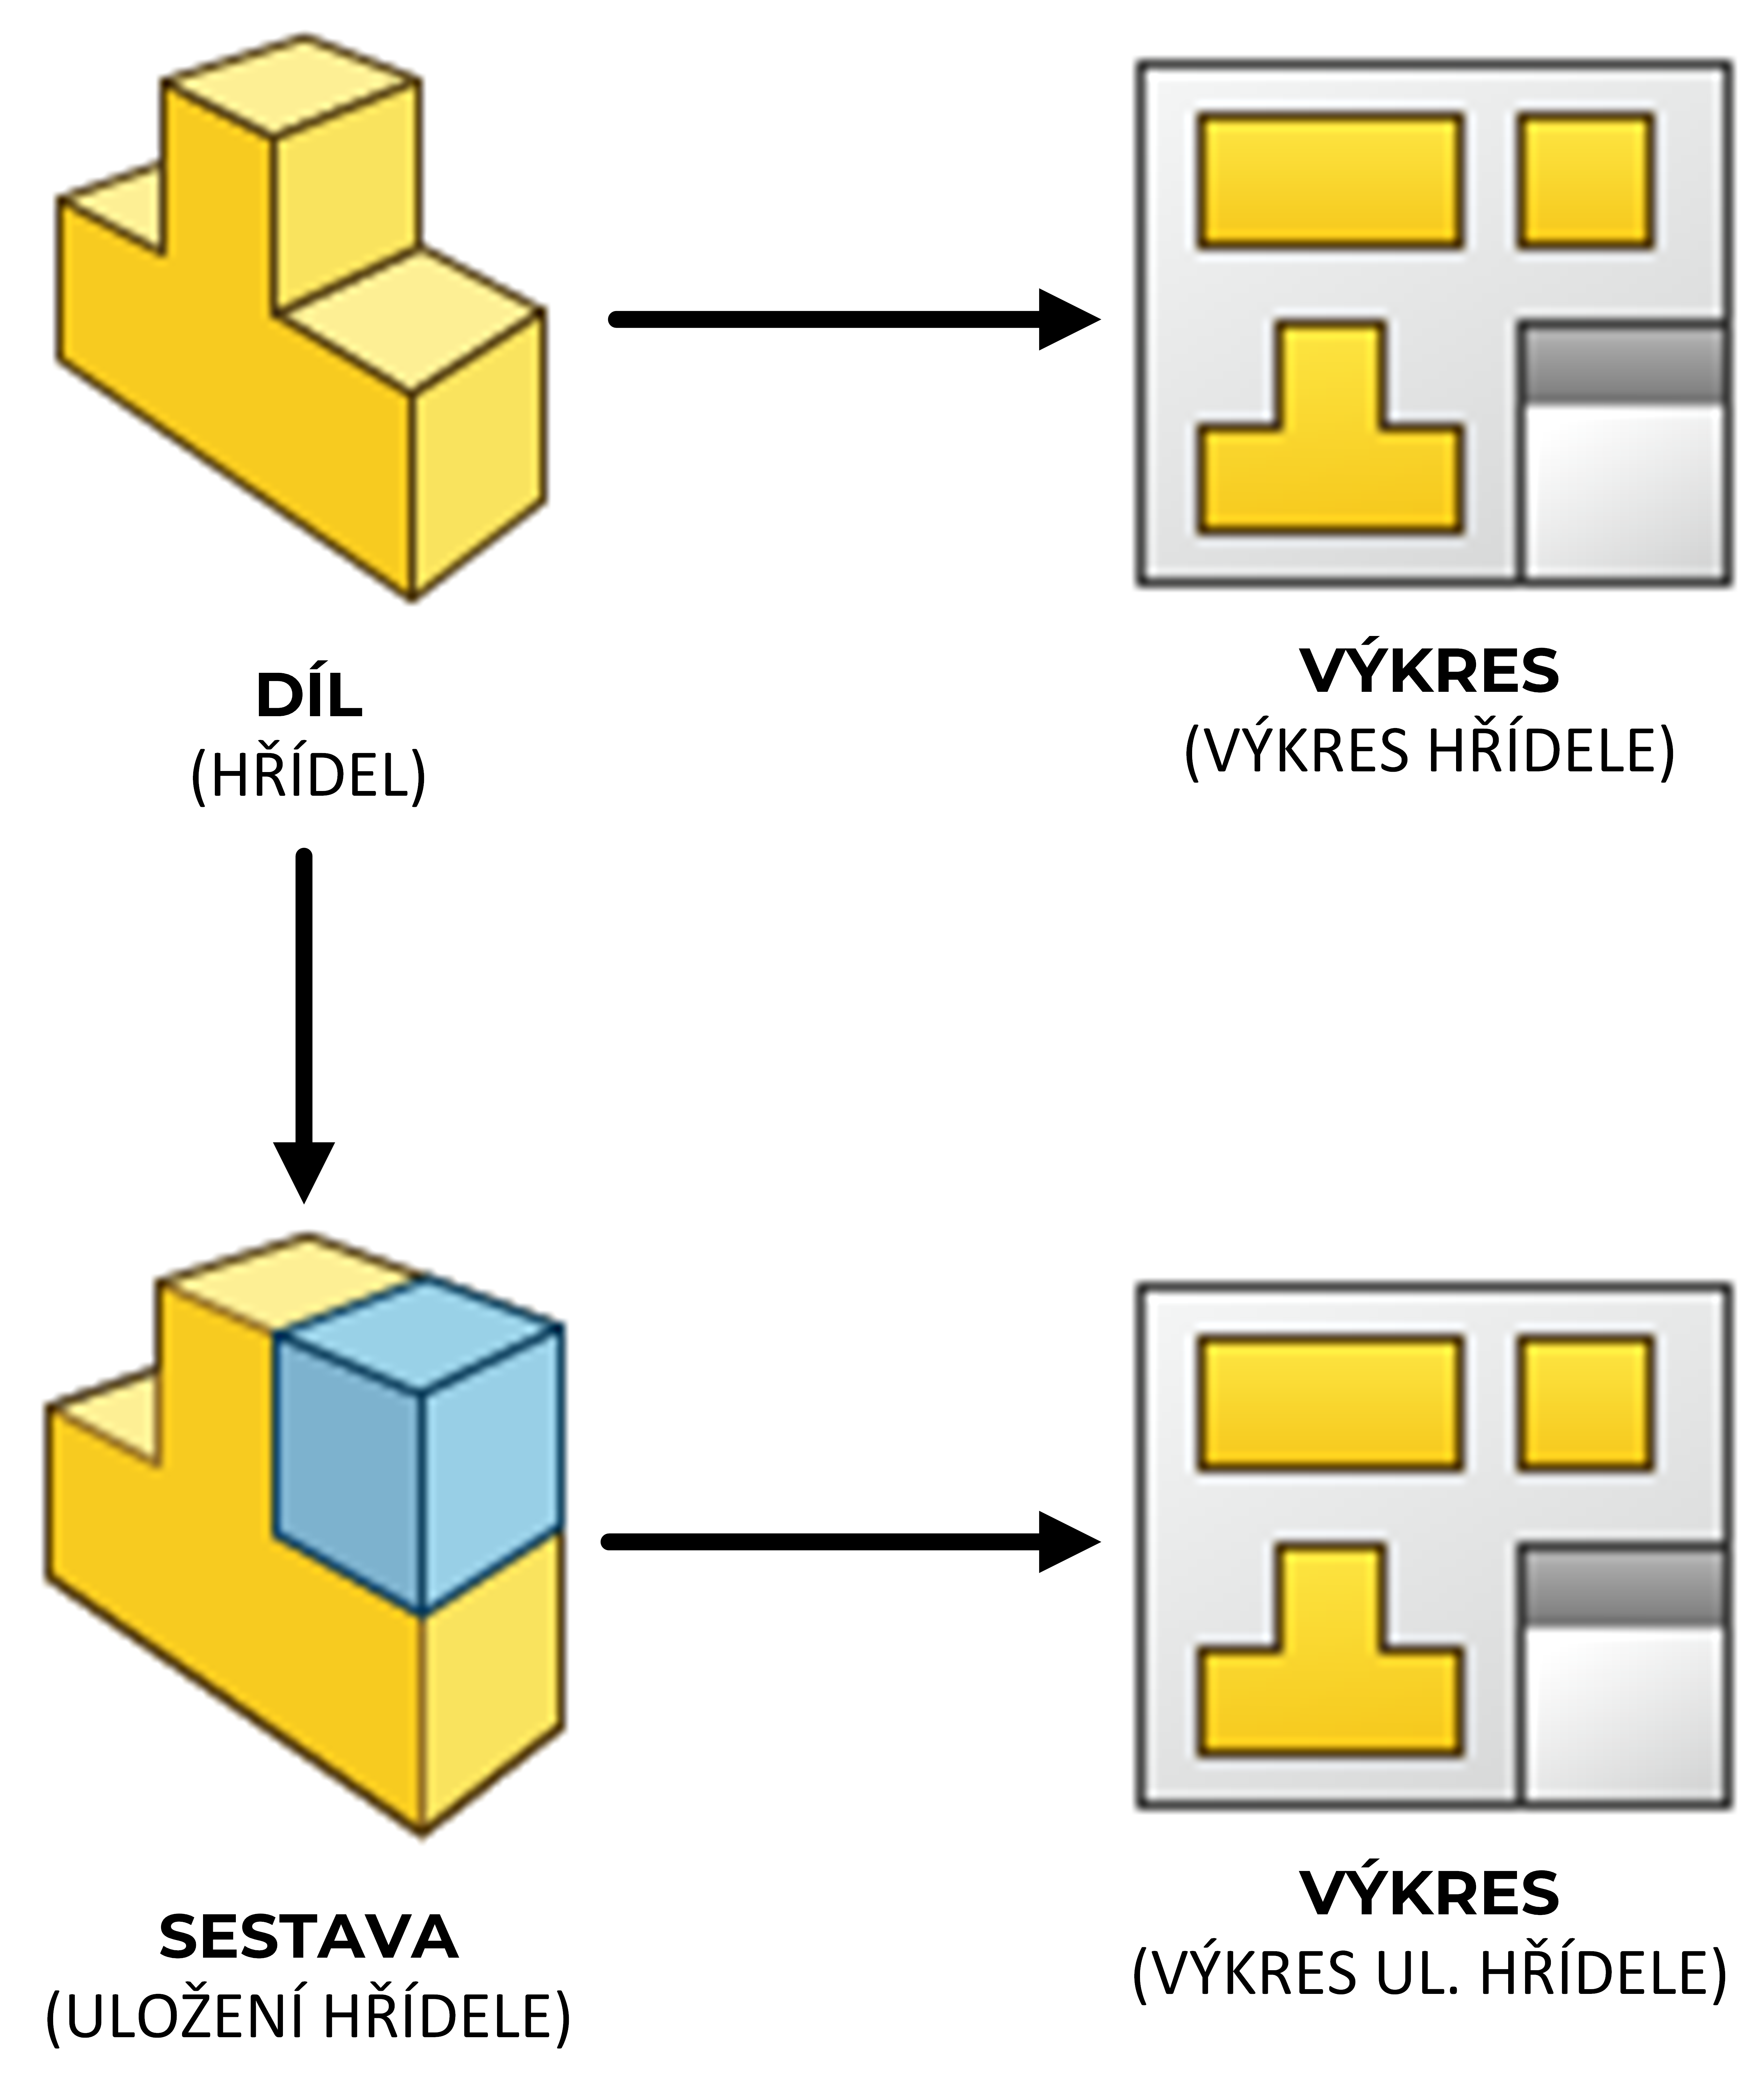
\includegraphics[width=0.35\textwidth]{img/graphics/png/SOLIDWORKS - PART-ASSEMBLY-DRAWING.png}
    \caption{Ilustrace vztahů mezi typy souborů SolidWorks}
    \label{fig:SOLIDWORKS_part-assembly-drawing}
\end{figure}

Pro to, abychom museli řešit přejmenovávání dílů v sestavách co nejméně, je dobré nazývat soubory správně již při vytváření.
Máme-li tedy nějaký díl (pro příklad vezměme ozubené kolo), pojmenujme jej tedy rovnou jako pastorek, nebo ozubené kolo.
Pokud již na začátku díl nazveme jako \enquote{kolečko}, \enquote{něco}, nebo zůstaneme u výchozího názvu \enquote{Díl1}, přijdeme později na to, že se v sestavě nedá orientovat, nebo že se v souborech nevyznáme.

\subsection*{Jak tedy na přejmenování dílu v sestavě?}
Prvoplánově může člověka napadnout si díl zobrazit v průzkumníkovi Windows, kliknout na něj pravým tl. myši a přejmenovat jej. 
Tím sice díl přejmenuje, ale všechny sestavy a výkresy, které na tento soubor před přejmenováním odkazovaly přestanou fungovat.

Správný postup je otevřít si sestavu, nebo výkres ve kterém se daný díl/sestava nachází a následně samotný díl, nebo sestavu, které chceme přejmenovat.
V nabídce \It{\enquote{Soubor}} u přejmenovávaného dílu/sestavy vybereme uložit jako a zvolíme první možnost - tedy uložení jako nový soubor s nahrazením vazeb.
Následně soubor uložíme s novým názvem, přepneme se na sestavu/výkres ve které je přejmenovaný díl obsažen, klikneme na tlačítko obnovit a na závěr sestavu/výkres uložíme.
Přejmenování je hotové a bez zbytečného rozbití vazeb.

\section{Jak správně přesunout sestavu na jiný počítač?}
S tímto problémem se setká každý strojař alespoň jednou.
Máte hotový projekt, tedy kompletní modely, výkresy, sestavu a chystáte se ji odevzdat.
Problém nastane ve chvílí, kdy 

%\newpage

% Uplatnění práce
\chapter{Uplatnění této práce}
Již v průběhu psaní této práce jsou videa, vytvořená v rámci tohoto projektu používána studenty Střední průmyslové školy v Brně na Sokolské.
Původně byla videa vytvořena primárně pro využití mezi studenty jakožto reference, pokud například zapomenou na způsob modelování nějakého prvku.
S postupným zavřením škol a zavedením distanční výuky našly videonávody uplatnění nejen, jako podpora studentů, ale i jako podpora samotné výuky konstruování.

Kromě studentů SPŠ a VOŠ Brno, Sokolská jsou videa P3D využívány i studenty jiných škol, včetně vysokoškoláků.

\newpage

\chapter{Další rozvoj projektu}


\newpage

% Zaver prace
\chapter*{Závěr}
\addcontentsline{toc}{chapter}{Závěr}
Sem přijde závěr práce.

\newpage
\newpage

\appendix
\addcontentsline{toc}{chapter}{Přílohy}

% Prilohy
\chapter{Seznam videí}
Tato příloha obsahuje kompletní seznam videí vzniklých v rámci projektu P3D vč. odkazů rozdělených dle jednotlivých témat. \newline
\noindent\It{Pozn.: při kliknutí na odkaz budete přesněrování na stránku korespondujícího videa}.

\section{Instalace a zprovoznění SolidWorks SDK}
\href{https://aka.parallaxproduction.cz/instalaceSDK}{Instalace a první spuštění SolidWorks SDK 2020/2021 (aka.parallaxproduction.cz/instSDK)} \newline
\href{https://aka.parallaxproduction.cz/sablony}{Instalace šablon a knihoven norm. dílů ze Sokolské (aka.parallaxproduction.cz/sablony)} \newline
\href{https://aka.parallaxproduction.cz/realview}{Aktivace Realview na necertifikované grafické kartě (aka.parallaxproduction.cz/realview)} \newline

\section{Základy modelování}
\href{https://aka.parallaxproduction.cz/jednoducha-pruzina}{Jednoduchá pružina (aka.parallaxproduction.cz/jednoducha-pruzina)} \newline
\href{https://aka.parallaxproduction.cz/j-ozubene-kolo}{Ozubené kolo s přímým čelním ozubením (aka.parallaxproduction.cz/j-ozubene-kolo)} \newline
\href{https://aka.parallaxproduction.cz/vyk-oz-kolo}{Ozubené kolo pro výkres - obálka (aka.parallaxproduction.cz/vyk-oz-kolo)} \newline
\href{https://aka.parallaxproduction.cz/jednorad-r-kolo}{Jednořadé řetězové kolo (aka.parallaxproduction.cz/jednorad-r-kolo)} \newline
\href{https://aka.parallaxproduction.cz/perodrazka-naboj}{Drážka pro pero v náboji (aka.parallaxproduction.cz/perodrazka-naboj)} \newline

\section{Výkresová dokumentace}


\section{Práce se sestavami}


\chapter{Obrazové přílohy}

%\begin{figure}[h]
%    \centering
%    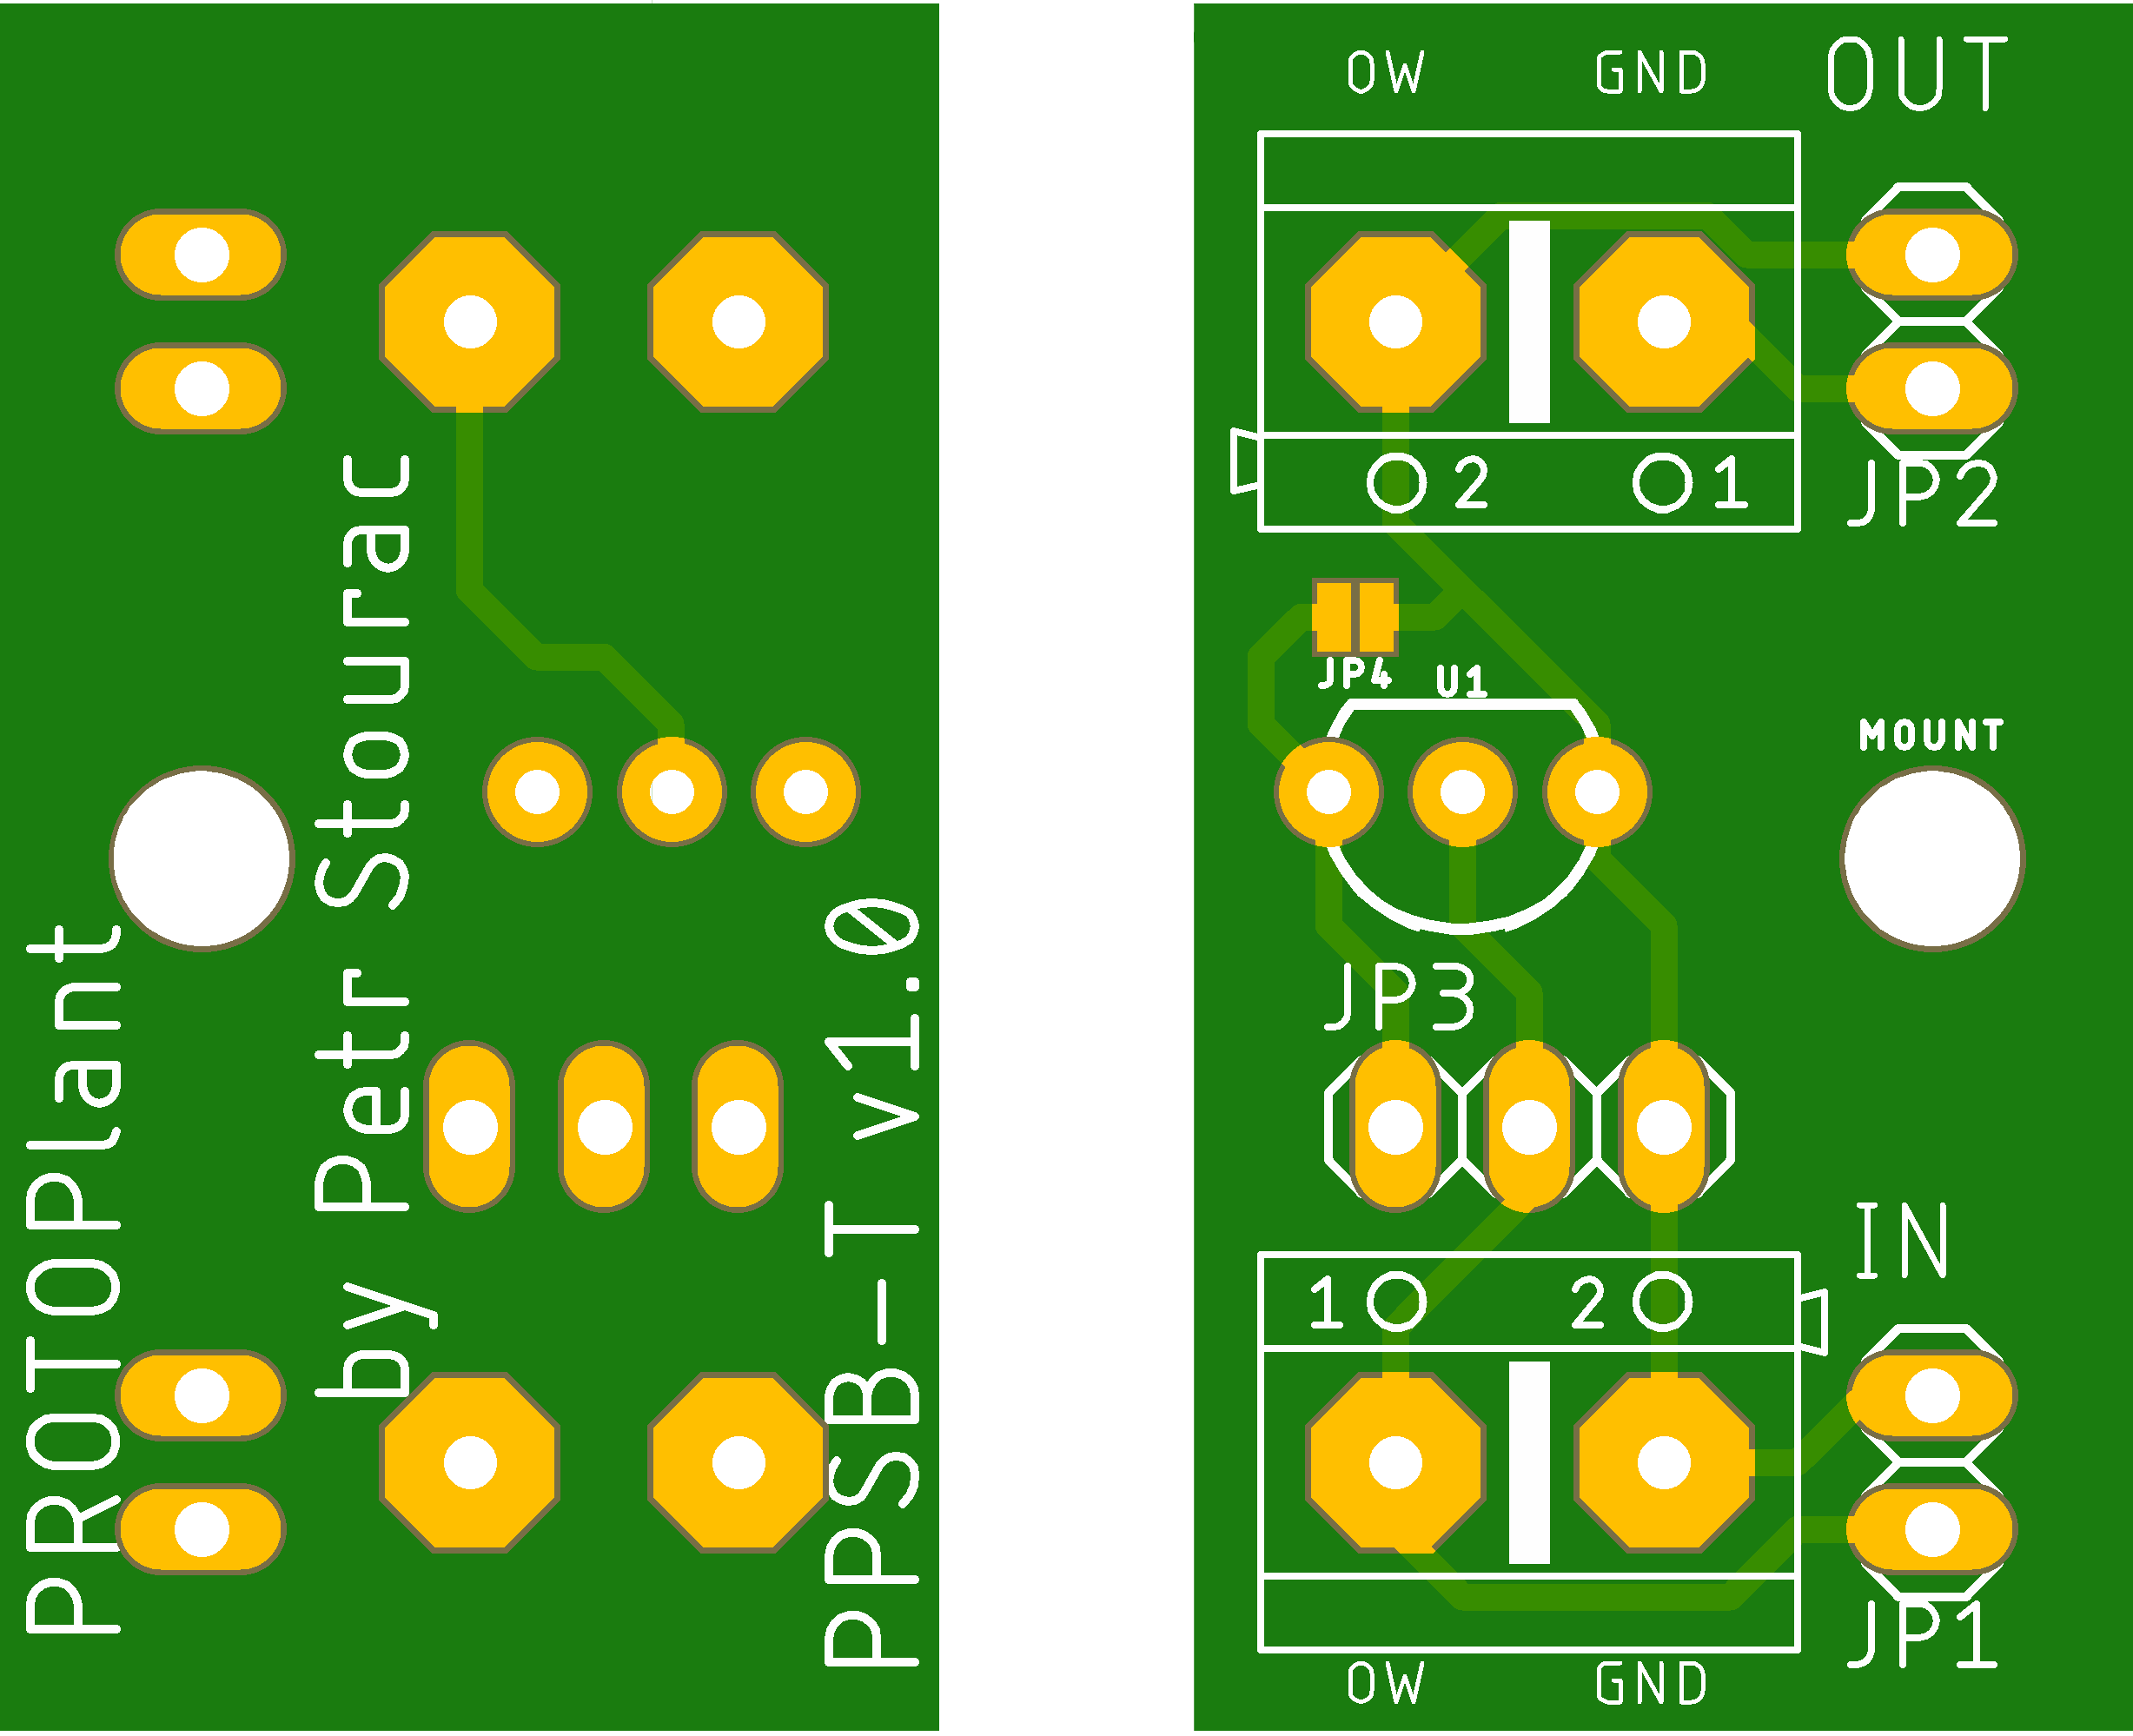
\includegraphics[width=0.85\textwidth]{img/ToBeRemoved/PPSB-T_BOTH.png}
%    \caption{Vizualizace PPSB-T (horní strana vpravo, dolní vlevo).}
%    \label{fig:PPSB-T_VISUAL}
%\end{figure}

% \printbibliography[title=Literatura]
\addcontentsline{toc}{chapter}{Literatura}

\listoffigures
\addcontentsline{toc}{section}{Seznam obrázků}

\listoftables
\addcontentsline{toc}{section}{Seznam tabulek}

\end{document}
